\documentclass[t, 10pt, mathserif]{beamer}

\usepackage[spanish]{babel}
\usepackage[utf8]{inputenc}
\usepackage{amscd}
\usepackage{amssymb}
\usepackage{amsthm}
\usepackage{latexsym}
\usepackage{setspace}
\usepackage{url}
\usepackage{xcolor}
\usepackage{bbm}

\mode<presentation>{
	\usecolortheme{}
	\useinnertheme{}
	\useoutertheme{}
}

\setbeamertemplate{caption}[numbered]
\setbeamertemplate{frametitle}[default][left,leftskip=0.5cm]
\setbeamersize{text margin left = 1cm}
\beamertemplatenavigationsymbolsempty
\addtobeamertemplate{frametitle}{\vspace*{0.5cm}}{\vspace*{1cm}}

\setlength{\parskip}{\baselineskip}
\expandafter\def\expandafter\item\expandafter{\item \setlength{\parskip}{0.5\baselineskip}}
\expandafter\def\expandafter\definition\expandafter{\definition \setlength{\parskip}{0.5\baselineskip}}

\languagepath{spanish}
\deftranslation[to=spanish]{Theorem}{Teorema}
\deftranslation[to=spanish]{theorem}{teorema}
\deftranslation[to=spanish]{Definition}{Definición}
\deftranslation[to=spanish]{definition}{definición}
\deftranslation[to=spanish]{Problem}{Problema}
\deftranslation[to=spanish]{problem}{problema}
\deftranslation[to=spanish]{Corollary}{Corolario}
\deftranslation[to=spanish]{corollary}{corolario}
\deftranslation[to=spanish]{Lemma}{Lema}
\deftranslation[to=spanish]{lemma}{lema}
\newtheorem{observation}{Observation}
\newtheorem{conjecture}{Conjecture}
\newtheorem{belief}{Belief}
\newtheorem{question}{Question}

\newcommand{\Z}{{\mathbb{Z}}}
\newcommand{\N}{{\mathbb{N}}}
\newcommand{\Q}{{\mathbb{Q}}}
\newcommand{\R}{{\mathbb{R}}}
\newcommand{\floor}[1]{\lfloor #1 \rfloor } 
\newcommand{\ceil}[1]{\lceil #1 \rceil }
\newcommand{\abs}[1]{\left| #1 \right|}
\newcommand{\card}{\mbox{\raisebox{.13em}{{$\scriptstyle \#$}}}}
\newcommand{\expa}[1]{\{#1\}}
\newcommand {\base}[2]{\langle{#1};{#2}\rangle}
\newcommand{\ybar}{{\overline{y}}}
\newcommand{\xbar}{{\overline{x}}}
\newcommand{\cf}{\text{\em cf}}
\newcommand{\eps}{\varepsilon}
\newcommand{\wh}[1]{\widehat{#1}}
\newcommand{\NN}{\mathbb{N}}
\newcommand{\RR}{\mathbb{R}}
\newcommand{\uno}{\mathbbm{1}}
\newcommand{\alocc}[2]{|\!|#1|\!|_{#2}}
\newcommand{\occ}[2]{|#1|_{#2}}

\author{\large Emilio Almansi}

\begin{document}

\title{\normalsize Tesis de Licenciatura en Ciencias de la Computación \vspace*{1.5cm}}

\subtitle{\Large Secuencias completamente equidistribuidas basadas en secuencias de De Bruijn}

\date{
  {\footnotesize
    \hspace*{-6cm}
    \begin{tabular}{l}
      Directora: Verónica Becher \\
      Departamento de Computación\\
      Facultad de Ciencias Exactas y Naturales\\
      Universidad de Buenos Aires\\
      4 de septiembre, 2019
    \end{tabular}
  }
}

%%%%%%%%%%%%%%%%%%%%%%%%%%%%%%%%%%%%%%%%%%%%%%%%%%%%%%%%%%%%%%%%%%%

\begin{frame}
  \vspace{0.5cm}
  \maketitle
  \setcounter{framenumber}{0}
  \thispagestyle{empty}
\end{frame}

%%%%%%%%%%%%%%%%%%%%%%%%%%%%%%%%%%%%%%%%%%%%%%%%%%%%%%%%%%%%%%%%%%%

\begin{frame}
  \frametitle{Sobre secuencias aleatorias}

  ¿Qué tienen en común las siguientes disciplinas?
  \pause

  \begin{itemize}
    \item Criptografía, seguridad informática.\pause
    \item Predicción del clima, medicina nuclear, simulación de proteínas.\pause
    \item Aprendizaje automático, algoritmos probabilistas.\pause
    \item Juegos de azar, videojuegos, deportes.
  \end{itemize}
  \pause

  {\color{orange} Generación de números aleatorios.}
  \pause

  Pero, ¿qué es una secuencia de números aleatorios?
\end{frame}

%%%%%%%%%%%%%%%%%%%%%%%%%%%%%%%%%%%%%%%%%%%%%%%%%%%%%%%%%%%%%%%%%%%

\begin{frame}
  \frametitle{Sobre secuencias aleatorias}

  \textbf{Intuición}: si tiro un dado muchas veces seguidas, el resultado de cada tirada tiene que ser \textit{impredecible} y cualquier número del 1 al 6 tiene que ser \textit{equiprobable}.
  \pause

  Respecto a la parte de \textit{impredecible}:
  \begin{quote}
    If ``random`` means that the sequence satisfies no predictable rules, the title of this paper is contradictory.
    \begin{flushright}
      \small{---Donald Knuth, 1965}
    \end{flushright}
  \end{quote}
  \pause

  En este trabajo, nos enfocamos en la parte de \textit{equiprobable}. \pause Es posible construir secuencias determinísticas que cumplen con esta propiedad.
\end{frame}

%%%%%%%%%%%%%%%%%%%%%%%%%%%%%%%%%%%%%%%%%%%%%%%%%%%%%%%%%%%%%%%%%%%

\begin{frame}
  \frametitle{Equidistribución}

  \begin{definition}
    Dado un entero $b$, una secuencia de \textit{números enteros} $x_1, x_2, \dots$ del conjunto $\{ 0, 1, \dots, b - 1 \}$ es \textbf{equidistribuida} si todo valor posible aparece con frecuencia asintótica igual a $\frac{1}{b}$:
    \pause

    \begin{equation*}
      \begin{aligned}
        Pr \left( x_i = j \right) = \frac{1}{b} \hspace*{1cm} \text{para } j = 0, \dots, b - 1 \text{,}
      \end{aligned}
    \end{equation*}

    donde $Pr(x_i = j) = \lim_{N \to \infty} \frac{1}{N} \sum_{i = 1}^{N} \sigma(x_i = j)$.
  \end{definition}
  \pause

  Ahora, definimos una noción equivalente para secuencias de números reales.
\end{frame}

%%%%%%%%%%%%%%%%%%%%%%%%%%%%%%%%%%%%%%%%%%%%%%%%%%%%%%%%%%%%%%%%%%%

\begin{frame}
  \frametitle{Equidistribución}

  \begin{definition}
    Una secuencia de \textit{números reales} $x_1, x_2, \dots$ en el intervalo unitario $\left[0, 1\right)$ es \textbf{equidistribuida} si la frecuencia de valores dentro de cualquier subconjunto $I$ es igual a su tamaño:
    \pause

    \begin{equation*}
      \begin{aligned}
        Pr \left( x_i \in I\, \right) = \left| I\, \right| \hspace*{1cm} \text{para todo } I \in \left[0, 1\right) \text{,}
      \end{aligned}
    \end{equation*}

    donde $Pr \left( x_i \in I\, \right) = \lim_{N \to \infty} \frac{1}{N} \sum_{i = 1}^{N} \sigma(x_i \in I\,)$.
  \end{definition}

\end{frame}

%%%%%%%%%%%%%%%%%%%%%%%%%%%%%%%%%%%%%%%%%%%%%%%%%%%%%%%%%%%%%%%%%%%

\begin{frame}
  \frametitle{Sobre secuencias aleatorias}

  \begin{figure}
    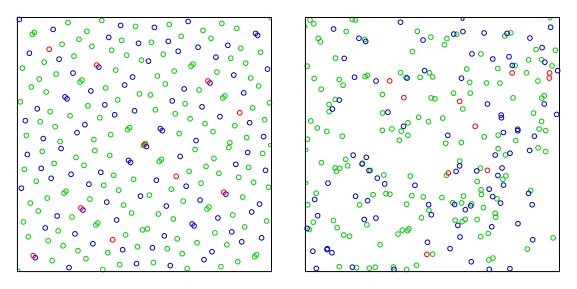
\includegraphics[width=\textwidth]{resources/discrepancia.png}
    \caption{Baja y alta discrepancia.}
  \end{figure}
\end{frame}
 
%%%%%%%%%%%%%%%%%%%%%%%%%%%%%%%%%%%%%%%%%%%%%%%%%%%%%%%%%%%%%%%%%%%

\begin{frame}
  \frametitle{Equidistribución completa}

  Aenean laoreet, ligula vel aliquet consectetur, mi magna rutrum urna, vel volutpat nulla purus sed lorem.
  \pause

  \medskip
  \begin{definition}
    Fusce sit amet lacus viverra, viverra massa sit amet, placerat neque. Integer ipsum sapien, efficitur quis dui vitae, facilisis tempus dolor.
    \pause

    Duis ornare volutpat libero, at sodales dolor porttitor at.
    \pause
  \end{definition}

  In rutrum dapibus justo, at mattis lacus ultrices sed. Suspendisse suscipit luctus fermentum.
\end{frame}


%%%%%%%%%%%%%%%%%%%%%%%%%%%%%%%%%%%%%%%%%%%%%%%%%%%%%%%%%%%%%%%%%%%

\begin{frame}
  \frametitle{Secuencias de De Bruijn}

  \medskip
  \begin{definition}[{{\scriptsize  Borel, 1909}}]
    Mauris euismod neque a lorem rutrum, id molestie eros consequat. In facilisis magna eu libero commodo, id tincidunt {\color{magenta} $\ell$} purus pellentesque:
    \begin{equation*}
      \lim_{n \rightarrow \infty} \frac{\alocc{u[1,\ell n]}{v}}{n} = \frac{1}{|A|^{\ell}}.  
    \end{equation*}
    \pause

    Donec nec ex id nisl venenatis semper. Curabitur erat mi, sagittis nec tortor vel, tempor porta magna. Cras at maximus orci, non viverra neque.
  \end{definition}
  \pause

  \medskip
  \begin{problem}[{{\scriptsize  Borel, 1909}}]
    In eget enim feugiat, cursus tellus eget, dapibus libero. Class aptent taciti sociosqu ad litora torquent per conubia nostra, per inceptos himenaeos.
  \end{problem}
\end{frame}

%%%%%%%%%%%%%%%%%%%%%%%%%%%%%%%%%%%%%%%%%%%%%%%%%%%%%%%%%%%%%%%%%%%

\begin{frame}
  \frametitle{La secuencia de Knuth (1)}

  Nam sagittis dolor in enim tincidunt, sit amet pellentesque urna.

  \begin{equation*}
    \begin{aligned}
      & F^{(2^n, n)}  & = \; & f_1, \dots, f_{2^{n^2}} \\[0.3cm]
      \pause
      & A^{(n)}       & = \; & \frac{f_1}{2^n}, \frac{f_2}{2^n}, \dots, \frac{f_{2^{n^2}}}{2^n} \\
      &               & = \; & \bigg( \frac{f_i}{2^n} \bigg)_{i = 1}^{2^{n^2}} \\[0.3cm]
      \pause
      & B^{(n)}       & = \; & \left< \underbrace{A^{(n)} ; A^{(n)} ; \dots ; A^{(n)}}_{n 2^{2 n} \text{ veces}} \right>
    \end{aligned}
  \end{equation*}
  \pause

  Porta purus neque, ultrices vulputate orci ullamcorper eu.
\end{frame}

  % \medskip
  % \begin{problem}
  %   Morbi euismod purus at cursus iaculis. Donec efficitur lorem rutrum, auctor justo id, rhoncus nibh.
  % \end{problem}
  % \pause

  % \medskip
  % \begin{theorem}[{{\scriptsize  Champernowne, 1933}}]
  %   Curabitur varius in ligula nec laoreet. Aenean ultricies eget mi quis maximus. Mauris ornare interdum vestibulum.
  % \end{theorem}

%%%%%%%%%%%%%%%%%%%%%%%%%%%%%%%%%%%%%%%%%%%%%%%%%%%%%%%%%%%%%%%%%%%

\begin{frame}
  \frametitle{La secuencia de Knuth (2)}

  For example, when $n = 2$:

  \begin{equation*}
    \begin{aligned}
      & F^{(4, 2)} = 0, 0, 1, 0, 2, 0, 3, 1, 1, 2, 1, 3, 2, 2, 3, 3 \\
      \pause
      & F^{(4, 2)} = 0, 0, 1, 0, 2, 0, 3, 1, 1, 2, 1, 3, 2, 2, 3, 3 \\
    \end{aligned}
  \end{equation*}
  % \begin{equation*}
  %   \begin{aligned}
  

  %     & B^{(2)} = \left< \underbrace{A^{(2)} ; \dots ; A^{(2)}}_{32 \text{ times}} \right> = \underbrace{\frac{0}{4}, \frac{0}{4}, \dots, \frac{3}{4}, \frac{3}{4}}_{A^{(2)}}, \dots, \underbrace{\frac{0}{4}, \frac{0}{4}, \dots, \frac{3}{4}, \frac{3}{4}}_{A^{(2)}}
  %   \end{aligned}
  % \end{equation*}
  % \pause

  and $|A^{(2)}| = 16$, $|B^{(2)}| = 512$.
\end{frame}

%%%%%%%%%%%%%%%%%%%%%%%%%%%%%%%%%%%%%%%%%%%%%%%%%%%%%%%%%%%%%%%%%%%

\begin{frame}
  \frametitle{La secuencia de Knuth (3)}

  Curabitur varius in ligula nec laoreet.
  \begin{equation*}
    K = \left< B^{(1)} ; B^{(2)} ;  B^{(3)} ; \dots \right>
  \end{equation*}
  \pause

  \medskip
  \begin{theorem}[{{\scriptsize  Knuth, 1965}}]
    Nam sagittis dolor in enim tincidunt, sit amet pellentesque urna vulputate.
  \end{theorem}
  \pause
  
  Morbi euismod purus at cursus iaculis. Donec efficitur lorem rutrum, auctor justo id, rhoncus nibh.
  \pause

  Aenean ultricies eget mi quis maximus. Mauris ornare interdum vestibulum.
\end{frame}

  % \medskip
  % \begin{problem}
  %   Morbi euismod purus at cursus iaculis. Donec efficitur lorem rutrum, auctor justo id, rhoncus nibh.
  % \end{problem}
  % \pause

%%%%%%%%%%%%%%%%%%%%%%%%%%%%%%%%%%%%%%%%%%%%%%%%%%%%%%%%%%%%%%%%%%%

\begin{frame}
  \frametitle{Tamaños de alfabeto linealmente crecientes}

  \medskip
  \begin{theorem}[{{\scriptsize  Agafonov 1968}}]
    Class aptent taciti sociosqu ad litora torquent per conubia nostra, per inceptos himenaeos
  \end{theorem}
  \pause

  \medskip
  \begin{corollary}
    Vestibulum quis dolor quam. Sed viverra, diam ac fringilla fringilla, ex dui consequat leo, nec tempus augue mi eu quam.
  \end{corollary}
  \pause

  \medskip
  \begin{theorem}[{{\scriptsize  Vandehey 2016}}]
    Phasellus quis aliquam nulla, non rutrum lorem. Class aptent taciti sociosqu ad litora torquent per conubia nostra, per inceptos himenaeos.
  \end{theorem}
\end{frame}

%%%%%%%%%%%%%%%%%%%%%%%%%%%%%%%%%%%%%%%%%%%%%%%%%%%%%%%%%%%%%%%%%%%

\begin{frame}
  \frametitle{Teorema principal}

  Nullam posuere tincidunt urna et elementum. Donec elementum at tellus sit amet tempus.
  \pause

  \medskip
  \begin{problem}
    Cras id accumsan risus, sed elementum elit. Suspendisse aliquet hendrerit gravida.
  \end{problem}
  \pause

  \medskip
  \begin{theorem}[\color{magenta} Resultado principal de esta tesis\color{black}]
    Nullam vehicula erat ante, hendrerit euismod elit luctus nec. Duis sagittis tincidunt metus, in dapibus lorem ullamcorper ut.
  \end{theorem}
\end{frame}

%%%%%%%%%%%%%%%%%%%%%%%%%%%%%%%%%%%%%%%%%%%%%%%%%%%%%%%%%%%%%%%%%%%

\begin{frame}
  \frametitle{Idea de la demostración}

  \medskip
  \begin{definition}
    Curabitur imperdiet tempus massa $A=\{0,1, \ldots, b-1\}$, pellentesque id turpis at mauris tempor auctor at pellentesque ex.
    \pause

    Pellentesque urna arcu, pellentesque sit amet volutpat eget, venenatis sed leo. Phasellus tempus eu urna a lacinia.
    \pause

    Vestibulum aliquam augue et tortor pulvinar suscipit $w^{\star}_n$.
    \pause

    Lorem ipsum dolor sit amet, consectetur adipiscing elit. Sed placerat nulla a vulputate ultrices. Ut et magna ac lacus elementum tincidunt a id ante.

    {\color{magenta}
      Donec $u=v_1 v_2 \ldots v_m$ aenean ullamcorper odio vitae $v_i$ erat $\ell_n$  rhoncus quis
      \[
      e_n(u)=e_n(v_1)\ldots e_n(v_m)
      \]
    }
  \end{definition}
\end{frame}

%%%%%%%%%%%%%%%%%%%%%%%%%%%%%%%%%%%%%%%%%%%%%%%%%%%%%%%%%%%%%%%%%%%

\begin{frame}
  \frametitle{Criterio de Weyl}

  \medskip
  \begin{definition}
    Suspendisse ut hendrerit $A$,  \textit{finibus semper neque non congue tortor dictum $\ell$} laoreet ex nec pulvinar $u\in A^*$ tellus
    \begin{equation*}
      \Delta_{A,\ell}(u) = 
      \max_{v \in A^{\ell}}\left(\left|\frac{\alocc{u}{v}}{\lfloor|u|/\ell \rfloor} - \frac{1}{|A|^{\ell}}\right|\right).
    \end{equation*}
  \end{definition}
  \pause

  Nam sagittis dolor in enim tincidunt $v\in A^\omega$ sit amet pellentesque urna vulputate $\ell$
  $$\lim_{n \rightarrow \infty} \Delta_{A, \ell}(v[1,\ell n]) = 0$$
\end{frame}


%%%%%%%%%%%%%%%%%%%%%%%%%%%%%%%%%%%%%%%%%%%%%%%%%%%%%%%%%%%%%%%%%%%

\begin{frame}
  \frametitle{Prueba alternativa}

  \medskip
  \begin{definition}
    Curabitur imperdiet tempus massa $A=\{0,1, \ldots, b-1\}$, pellentesque id turpis at mauris tempor auctor at pellentesque ex.
    \pause

    Pellentesque urna arcu, pellentesque sit amet volutpat eget, venenatis sed leo. Phasellus tempus eu urna a lacinia.
    \pause

    Vestibulum aliquam augue et tortor pulvinar suscipit $w^{\star}_n$.
    \pause

    Lorem ipsum dolor sit amet, consectetur adipiscing elit. Sed placerat nulla a vulputate ultrices. Ut et magna ac lacus elementum tincidunt a id ante.

    {\color{magenta}
      Donec $u=v_1 v_2 \ldots v_m$ aenean ullamcorper odio vitae $v_i$ erat $\ell_n$  rhoncus quis
      \[
      e_n(u)=e_n(v_1)\ldots e_n(v_m)
      \]
    }
  \end{definition}
\end{frame}

%%%%%%%%%%%%%%%%%%%%%%%%%%%%%%%%%%%%%%%%%%%%%%%%%%%%%%%%%%%%%%%%%%%

\begin{frame}
  \frametitle{Problemas abiertos}

  Cras id accumsan risus, sed elementum elit.
  \pause

  \begin{itemize}
    \item Donec eu sollicitudin lacus. Vestibulum facilisis eu tellus quis gravida. Proin faucibus tellus nec tempus maximus.
    \pause
    
    \item Proin at facilisis orci. Nunc at orci in ante semper elementum ullamcorper in est. Praesent maximus aliquet lorem, in tincidunt odio tempus vel.
    \pause

    \item Etiam vulputate nunc eget mauris vestibulum, nec viverra massa lacinia. Donec volutpat tempus nunc, vitae malesuada odio ultricies nec. 
  \end{itemize}
\end{frame}

\newcounter{finalframe}
\setcounter{finalframe}{\value{framenumber}}

\addtocounter{framenumber}{-1}

% \begin{frame}
% \scriptsize

% \begin{thebibliography}{1}

% \setlength{\parskip}{-0.5mm}

% \bibitem{agafonov1968normal}
% V.~N. Agafonov.
% \newblock Normal sequences and finite automata.
% \newblock {\em Soviet Mathematics Doklady}, 9:324--325, 1968.

% \bibitem{BecherCarton2017}
% Ver\'onica Becher and Olivier Carton.
% \newblock Normal numbers and computer science.
% \newblock In Val\'erie Berth\'e and Michel Rig\'o, editors, {\em Sequences,
%   Groups, and Number Theory}, Trends in Mathematics Series.
%   Birkhauser/Springer, 2017.

% \bibitem{borel1909probabilites}
% {\'E}mile Borel.
% \newblock Les probabilit{\'e}s d{\'e}nombrables et leurs applications
%   arithm{\'e}tiques.
% \newblock {\em Rendiconti del Circolo Matematico di Palermo}, 27(1):247--271,
%   1909.

% \bibitem{bugeaud2012distribution}
% Yann Bugeaud.
% \newblock {\em Distribution modulo one and Diophantine approximation}, volume
%   193.
% \newblock Cambridge University Press, 2012.

% \bibitem{Champernowne:1933}
% David Champernowne.
% \newblock The {C}onstruction of {D}ecimals {N}ormal in the {S}cale of {T}en.
% \newblock {\em The Journal of the London Mathematical Society},
%   s1-8(4):254--260, 1933.

% \bibitem{rogers1987theory}
% Jr. Hartley~Rogers.
% \newblock {\em Theory of recursive functions and effective computability}.
% \newblock MIT Press, Cambridge, MA, second edition, 1987.

% \bibitem{kamae1975normal}
% Teturo Kamae and Benjamin Weiss.
% \newblock Normal numbers and selection rules.
% \newblock {\em Israel Journal of Mathematics}, 21(2):101--110, 1975.

% \bibitem{Piatetski-Shapiro:1951}
% I.~I. Piatetski-Shapiro.
% \newblock On the law of distribution of the fractional parts of the exponential
%   function.
% \newblock {\em Izv. Akad. Nauk SSSR Ser. Mat.}, 15(1):47--52, 1951.

% \bibitem{vandehey2016uncanny}
% Joseph Vandehey.
% \newblock Uncanny subsequence selections that generate normal numbers.
% \newblock {\em ar{X}iv:1607.03531}, 2016.
% \end{thebibliography}

% \end{frame}

\end{document}
